%\documentclass[a4 paper,12pt]{report}
\documentclass[a4 paper,12pt,ukrainian]{report}
\usepackage[12pt]{extsizes}
\usepackage[utf8]{inputenc}
%\usepackage[utf8]{inputenc}
\usepackage[ukrainian]{babel}
\usepackage{amsfonts,amsmath}
\usepackage[pdftex]{graphicx}
%\usepackage{amsthm}
\usepackage{makeidx,bezier,latexsym,epsfig,layout}
\textheight 22.5 cm \textwidth 16 cm \topmargin -1 cm
\evensidemargin 0 cm \oddsidemargin 0 cm
\newtheorem{theorem}{\textbf{Теорема}}[chapter]
%\newtheorem{proof}{\textbf{Дов.:}}
\newtheorem{lema}[theorem]{\textbf{Лема}}
\newtheorem{determination}[theorem]{\textbf{Означення}}
\begin{document}
%!!!!!!!!!!!!!!!!!!!!!!!! титульна !!!!!!!!!!!!!!!!!!!!!
\titlepage
\begin{center}
\large {Міністерство освіти та науки України}\\
\large {Львівський національний університет імені Івана Франка}\\
\large {Факультет прикладної математики та інформатики}\\
\end{center}

\normalsize \vspace*{2cm}
\hspace*{11cm}Допущено до захисту\\
\hspace*{11cm}Завідувач кафедри\\
\hspace*{11cm}\underline{\hspace{3cm}}\\
\hspace*{11cm}проф. Хапко Р.С.\\
\hspace*{11cm}"\underline{\hspace{0.5cm}}"\underline{\hspace{2cm}} 2016 р.
\normalsize \vspace*{2cm}
\begin{center}
\large{Роман Андрій}\\
\large{Зварич Андрій}\\
\large{\textbf{Чисельне розв'язування мішаної задачі для рівнняння Лапласа методом ІР}}\\
\large{Звіт}\\
\end{center}
\normalsize \vspace*{3cm}
\hspace*{11cm}Наукові консультанти\\
\hspace*{11cm}проф. Р. Хапко\\
\hspace*{11cm}ст.викл. Я. Гарасим\\
\hspace*{11cm}асист. В. Вавричук\\
\\
\\
\\
\\
\\
\\
\large\centerline{Львів 2016}
%!!!!!!!!!!!!!!!!!!!!!!!!сторінка змісту!!!!!!!!!!!!!!!!!!!!!
\tableofcontents
%!!!!!!!!!!!!!!!текст курсової!!!!!!!!!!!!!!!!!!!!!!!!
\chapter*{\bf{Вступ}}
\addcontentsline{toc}{chapter}{Вступ}
\hspace*{\parindent}Дослiдження граничних задач для рiвнянь в частинних похiдних є однiєю з
найважливiших сфер застосування методу iнтегральних рiвнянь. Цей метод має низку
незаперечних переваг у порiвняннi з iншими методами, а саме: зменшення розмiрностi
задачi на одиницю, застосовнiсть для областей з границями довiльної форми i частково
необмежених областей, наближений роз'язок точно задовольняє диференційне рівняння.\\
\hspace*{\parindent}Метою даної роботи є навчитися чисельно розв’язувати крайовi задачi для
рiвняння Лапласа у обмеженій області. Планується довести єдинiсть класичного
розв’язку поставленої задачi. Будемо застосовувати непрямий метод iнтегральних рiвнянь. Також потрiбно
з’ясувати коректнiсть отриманого iнтегрального рiвняння, здiйснити
параметризацiю iнтегрального рiвняння i видiлення особливостi.\\
\hspace*{\parindent}Наближений розв’язок iнтегрального рiвняння будемо знаходити задопомогою тригонометричних квадратур. Потрiбно довести збiжнiсть методу i
знайти апрiорну оцiнку похибки, а також наближений розв’язок диференцiальної задачi.
\chapter{Загальні відомості}
\section{Постановка задачі}
\hspace*{\parindent}Нехай $D_0\subset \mathbb{R}^2$ - круг радіуса $R>0$ з границею $\Gamma_0$, $D_1\subset D_0$ і $D_2\subset D_0$ - області з границями $\Gamma_i\in C^2$, $i=1,2$. Причому $D_1\cap D_2=\{\emptyset\}$.\\ 
\hspace*{\parindent}Позначимо $D=D_0\setminus (\bar{D_1}\cup\bar{D_2})$. Необхідно знайти функцію $u:D \rightarrow \mathbb{R}$, яка задовольняє рівняння Лапласа
\begin{equation}
\Delta u=0\text{ в }D
\end{equation}
і граничні умови 

\begin{equation}
		u = f_2 \mbox{  на  }  \Gamma_2 ,\quad
		\frac{\partial u}{\partial \nu} = f_1 \mbox{  на  }  \Gamma_1 ,\quad
		\frac{\partial u}{\partial \nu} = f_0 \mbox{  на  } \Gamma_0 ,\quad
\end{equation}

Тут $f_0$, $f_1$, $f_2$ - задані функції.
\begin{figure}[htb]
\center{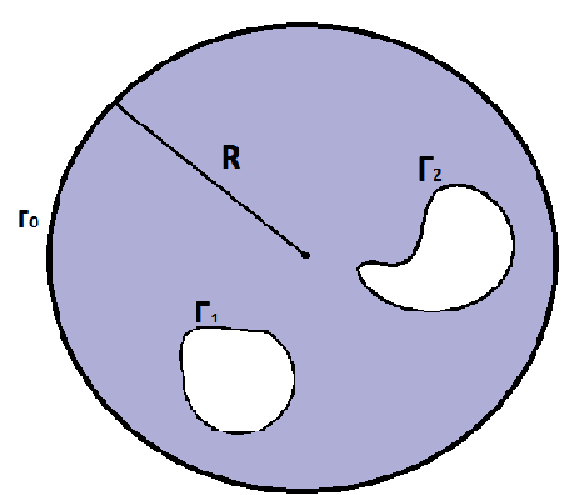
\includegraphics[scale=0.5]{draw}}%[scale=0.8]
\caption{Геометрія області}
\label{fig:image}
\end{figure}

%####################################################################################################################################################################################################################################################################################################################################################################################################################

\section{Єдиність класичного розв'язку задачі}
\begin{determination}
Двічі неперервно-диференційовна дійснозначна функція $u\in C^2(D)$, визначена в $D\subset\mathbb{R}^2$, називається гармонічною, якщо вона задовольняє рівняння Лапласа (1.1).
\end{determination}
\begin{theorem}
Задача (1.1)-(1.2) має щонайбільше один розв'язок.
\end{theorem}
\textbf{Дов.}(Від супротивного). Нехай існують дві гармонічні функції $u_1$, $u_2$, які є різними розв'язками задачі (1.1)-(1.2). Очевидно, що $u=u_1-u_2$ - також гармонічна функція, яка рівна нулю на границі $D$ (оскільки $u_1=u_2$ на $\partial D$).\\
\hspace*{\parindent}Використавши першу теорему Гріна [1]:
\begin{equation*}
\int\limits_{D}\left\{u \ \Delta v+gradu\cdot gradv\right\}dx=\int\limits_{\partial D}u\frac{\partial v}{\partial\nu}ds,
\end{equation*}
де $\nu$ - зовнішня нормаль. При $u=v$ маємо:
\begin{equation*}
u \ \Delta u=0 \quad (\Delta u=0\text{ в }D)
\end{equation*}
\begin{equation*}
u\frac{\partial v}{\partial\nu}=0 \quad (u=0\text{ на }\partial D)
\end{equation*}
\begin{equation*}
\Rightarrow\int\limits_{D}gradu\cdot gradu \ dx=0
\end{equation*}
\begin{equation*}
\int\limits_{D}\Bigl(\frac{\partial u}{\partial x_1},\frac{\partial u}{\partial x_2}\Bigr)\cdot\Bigl(\frac{\partial u}{\partial x_1},\frac{\partial u}{\partial x_2}\Bigr)dx=\int\limits_{D}\left\{\Bigl(\frac{\partial u}{\partial x_1}\Bigr)^2+\Bigl(\frac{\partial u}{\partial x_2}\Bigr)^2\right\}dx=0
\end{equation*}
\begin{equation*}
\Rightarrow \ \frac{\partial u}{\partial x_1}=0, \quad \frac{\partial u}{\partial x_2}=0 \ \Rightarrow \ u=const.
\end{equation*}
Оскільки на $\partial D \ u=0$, то: $ \ u\equiv 0 \ \Rightarrow \ u_1=u_2$ - суперечність. $\quad\quad\quad\Box$ 
\newpage



%####################################################################################################################################################################################################################################################################################################################################################################################################################


\section{Потенціали та їх властивості}
\begin{determination}
Нехай задана функція $\varphi\in C(\partial D)$, $D\subset\mathbb{R}^m$ - деяка область. Функції
\begin{equation*}
u(x) = \int\limits_{\partial{D}} \, \varphi(y)N(x,y) ds(y) , \quad x \in \mathbb{R}^m\setminus D
\end{equation*}
та
\begin{equation*}
\upsilon(x) = \int\limits_{\partial{D}} \, \varphi(y)\frac{\partial N(x,y)}{\partial\nu(y)} ds(y) , \quad x \in \mathbb{R}^m\setminus D
\end{equation*}
називають відповідно потенціалом простого шару і потенціалом подвійного шару з неперервною густиною $\varphi$.
\end{determination}
\hspace*{\parindent}Для розв'язування граничних задач за допомогою потенціалів, необхідно дослідити їхню поведінку на границі $\partial{D}$, тому доцільно ввести наступні твердження.
\begin{theorem}
Нехай $\partial{D}\in C^2$, $\varphi\in C(\partial{D})$. Тоді потенціал простого шару $u$ з густиною $\varphi$ є неперервним в $\mathbb{R}^m$. На границі маємо:
\begin{equation*}
u(x) = \int\limits_{\partial{D}} \, \varphi(y)N(x,y) ds(y) , \quad x \in \partial D,
\end{equation*}
де інтеграл існує як невласний.
\end{theorem}
\begin{theorem}
Нехай $\partial D\in C^2$ і $\varphi\in C(\partial D)$. Тоді потенціал подвійного шару $\upsilon$ з густиною $\varphi$ може бути неперервно продовжений з $D$ до $\bar{D}$ і з $\mathbb{R}^m\setminus\bar{D}$ до $\mathbb{R}^m\setminus D$ з граничними значеннями
\begin{equation*}
\upsilon_\pm(x) = \pm\frac{1}{2}\varphi(x)+\int\limits_{\partial{D}} \, \varphi(y)\frac{\partial N(x,y)}{\partial\nu(y)} ds(y) , \quad x \in \partial D,
\end{equation*}
де $\upsilon_\pm(x)=\lim\limits_{h \to 0}\upsilon(x\pm h\nu(x))$ і інтеграли існують як невласні. 
\end{theorem}
\begin{theorem}
Нехай $\partial D\in C^2$ і $\varphi\in C(\partial D)$. Тоді для потенціалу простого шару $u$ з густиною $\varphi$ маємо:
\begin{equation*}
\frac{\partial u_\pm}{\partial\nu}(x)=\mp\frac{1}{2}\varphi(x)+\int\limits_{\partial D}\varphi(y)\frac{\partial N(x,y)}{\partial\nu(x)} ds(y) , \quad x \in \partial D,
\end{equation*}
де $\frac{\partial u_\pm}{\partial\nu}(x)=\lim\limits_{h \to 0}\nu(x)\cdot gradu(x\pm h\nu(x))$ і інтеграли існують як невласні.
\end{theorem}
%####################################################################################################################################################################################################################################################################################################################################################################################################################



\chapter{Чисельне розв'язування крайової задачі}
\section{Інтегральне подання розв'язку}
\hspace*{\parindent}Фундаментальним розв'язком задачі (1.1)-(1.2) є функція Гріна задачі Неймана для рівняння Лапласа в крузі $D_{0}\subset{\mathbb{R}^2}$ з радіусом $R$ для усіх $x\not=y$ в $\bar{D_{0}}$ 
\begin{equation*}
N(x,y) = \frac{1}{2\pi} \ln{\frac{1}{|x-y|}} + \tilde{N}(x,y),
\end{equation*}
де
\begin{equation*}
\tilde{N}(x,y) = \frac{1}{2\pi}\ln{\bigg(\bigg|y-\frac{xR^2}{|x|^2}\bigg|\frac{|x|}{R^3}\bigg)}.
\end{equation*}
\hspace*{\parindent}Подамо розв'язок задачі (1.1)-(1.2) у вигляді:
\begin{equation}
\ u(x)=u_{1}(x)+u_{2}(x),
\end{equation}
де $u_{1}(x)$ - розв'язок задачі:
\begin{equation}
 \begin{cases}
   \Delta{u_{1}} = 0 \quad \textup{в} \quad D_{0},
   \\
   \frac{\partial u_{1}}{\partial\nu} = f_{0}  \quad \textup{на} \quad \Gamma_{0},
 \end{cases}
\end{equation}
$u_{2}(x)$ - розв'язок задачі:
\begin{equation}
 \begin{cases}
   \Delta{u_{2}} = 0 \quad \textup{в} \quad D_{0} \backslash({D_{1}}\cup {D_{2}})%D_1\bigcup D_2,
   \\
   u_{2}=0 \quad \textup{на} \quad \Gamma_{0},
	\\
   \frac{\partial u_{2}}{\partial\nu} = f_{1} - \frac{\partial u_{1}}{\partial\nu} \quad \textup{на} \quad \Gamma_{1},
	\\
   u_{2} = f_{2} - u_{1} \quad \textup{на} \quad \Gamma_{2},

 \end{cases}
\end{equation}
\hspace*{\parindent}Розв'язком задачі (2.2) є інтеграл вигляду:
\begin{equation}
u_{1}(x) = \int\limits_{\Gamma_{0}} \, f_{0}(y)N(x,y) ds(y). 
\end{equation}
\hspace*{\parindent}Розв'язок задачі (2.3):
\begin{equation}
u_{2}(x) = \int\limits_{\Gamma_{1}} \, \varphi_{1}(y)N(x,y)ds(y)+\int\limits_{\Gamma_{2}} \, \varphi_{2}(y)\bigg(\frac{\partial N(x,y)}{\partial\nu} + 1\bigg)ds(y). 
\end{equation}
\hspace*{\parindent}Тоді розв'язок задачі (1.1)-(1.2) можна подати у вигляді лінійної комбінації потенціалів:
\begin{equation}
u(x) = \int\limits_{\Gamma_{1}} \, \varphi_{1}(y)N(x,y)ds(y)+\int\limits_{\Gamma_{2}} \, \varphi_{2}(y)\bigg(\frac{\partial N(x,y)}{\partial\nu} + 1\bigg)ds(y)+
\end{equation}
\begin{equation*}
+\int\limits_{\Gamma_{0}} \, f_{0}(y)N(x,y) ds(y), \quad x \in D,
\end{equation*}
де густини $\varphi_{1}$, $\varphi_{2}$ визначаються з системи інтегральних рівнянь другого роду:
\begin{equation}\label{13}
 \left\{
\begin{array}{c}
   \displaystyle
\frac{1}{2}\varphi_{1}(x) + \int\limits_{\Gamma_1} \, \varphi_1(y)N(x,y)ds(y)+\int\limits_{\Gamma_2} \, \varphi_2(y)\bigg(\frac{\partial N(x,y)}{\partial\nu} + 1\bigg)ds(y)=f_1(x)-\frac{\partial u_{1}(x)}{\partial\nu},\\ \quad x\in \Gamma_1,\\

	\displaystyle
  -\frac{1}{2}\varphi_{2}(x) + \int\limits_{\Gamma_1} \, \varphi_1(y)N(x,y)ds(y)+\int\limits_{\Gamma_2} \, \varphi_2(y)\bigg(\frac{\partial N(x,y)}{\partial\nu} + 1\bigg)ds(y)=f_2(x)-u_{1}(x),\\ \quad x\in \Gamma_2,
 \end{array}
\right.
\end{equation}


%########################################################################################################################################################################################################################################################################################################################################################################################################################################################################
%ПОМІНЯТИ!!!!!!!!!!!!!!!!!!!!!!!!!!!!!!!!!!!!!!!!!!!!!!!!!!!!!!!!!!!!!!!!!!!!!!!!!!!!!!!!!!!!!!
\newpage
\section{Коректність отриманих інтегральних рівнянь}
\begin{theorem}
Потенціал подвійного шару з $\varphi \in C(\partial D)$
\begin{equation*}
u(x) = \int\limits_{\partial D} \, \varphi(y) \bigg(\frac{\partial F(x,y)}{\partial \nu} + \frac{1}{|x|^{m-2}}\bigg)ds(y), x \in R^m \setminus D
\end{equation*}
\\ з $\varphi$ є розв'язком зовнішьої задачі Діріхле, якщо $\varphi$ є розв'язком інтегрального рівняння другого роду.
\begin{equation}
\varphi(x) + 2\int\limits_{\partial D} \, \varphi(y) \bigg(\frac{\partial F(x,y)}{\partial \nu} + \frac{1}{|x|^{m-2}}\bigg)ds(y) = 2f(x), x \in R^m \setminus D
\end{equation}
\end{theorem}

\begin{theorem}
Зовнішня задача Діріхле має щонайбільше один розв'язок.
\end{theorem}


\begin{theorem}
Потенціал простого шару з $\varphi \in C(\partial D)$
\begin{equation*}
u(x) = \int\limits_{\partial D} \, \varphi(y) F(x,y)ds(y), x \in  D
\end{equation*}
\\ з $\varphi$ є розв'язком внутрішньої задачі Неймана, якщо $\varphi$ є розв'язком інтегрального рівняння другого роду.
\begin{equation}
\varphi(x) + 2\int\limits_{\partial D} \, \varphi(y) (\frac{\partial F(x,y)}{\partial \nu})ds(y) = 2f(x), x \in \partial D
\end{equation}
\end{theorem}

\begin{theorem}
Два розв'язки внутрішньої задачі Неймана відрізняютсья на константу.
Зовнішня задача Неймана має найбільше один розв'язок.
\end{theorem}

\begin{theorem}
Внутрішня задача Неймана є розв'язною тоді і лише тоді, якщо
\begin{equation*}
\int\limits_{\partial D} \, f(y)ds(y) = 0
\end{equation*}
\end{theorem}



\begin{theorem}
Потенціал простого шару з $\varphi \in C(\partial D)$
\begin{equation*}
u(x) = \int\limits_{\partial D} \, \varphi(y) F(x,y)ds(y), \varphi \in R^m \setminus D
\end{equation*}
\\ з $\varphi$ є розв'язком зовнішньої задачі Неймана, якщо $\varphi$ є розв'язком інтегрального рівняння другого роду.
\begin{equation}
\varphi(x) - 2\int\limits_{\partial D} \, \varphi(y) (\frac{\partial F(x,y)}{\partial \nu})ds(y) = -2f(x), x \in \partial D
\end{equation}
та при m = 2 :
\begin{equation}
\int\limits_{\partial D} \, \varphi(y) ds(y) = 0
\end{equation}
\end{theorem}
%################################################################################################################################################################################################################################################################################################################################################################################################################################################################
\section{Параметризація та виділення особливості}
\hspace*{\parindent}Нехай границі $\Gamma_{0}$, $\Gamma_{1}$ та $\Gamma_{2}\in C^{2}$ задаються параметрично:
\begin{equation*}
\Gamma_i :=\{x_i(t) = (x_i_1(t),x_i_2(t)), t \in [0,2\pi]\}, i=0,1,2.
\end{equation*}
Тут $x_{i}: [0,2\pi]\to\mathbb{R}^{2}\in C^{2}[0,2\pi]-2\pi$-періодична функція, для якої $|x_{i}'(t)|>0$, $t\in[0,2\pi]$.\\ 
\hspace*{\parindent}Тоді систему інтегральних рівнянь (2.7) можна подати в параметричному вигляді:
\begin{equation}
\left\{
\begin{array}{c}
\displaystyle
\frac{1}{2}\mu_1(t) + \frac{1}{2\pi}\int\limits_{0}^{2\pi} \, \mu_1 (\tau)H_{1}(t,\tau)d\tau+\frac{1}{2\pi}\int\limits_{0}^{2\pi} \, \mu_2 (\tau)\bigg(\frac{\partial L_1(t,\tau)}{\partial\nu} + 1\bigg)d\tau=g_1(t),\\ t\in [0, 2\pi]\\
\displaystyle
-\frac{1}{2}\mu_2(t) + \frac{1}{2\pi}\int\limits_{0}^{2\pi} \, \mu_1 (\tau)L_{2}(t,\tau)d\tau+\frac{1}{2\pi}\int\limits_{0}^{2\pi} \, \mu_2 (\tau)\bigg(\frac{\partial L_1(t,\tau)}{\partial\nu} + 1\bigg)d\tau=g_2(t),\\ t\in [0, 2\pi]
\end{array}
\right.
\end{equation}
де 
\begin{equation*}
\mu_{i}(t)=\varphi(x_{i}(t)) -2\pi\textup{-періодична функція}, \quad i=1,2,
\end{equation*}
\begin{equation*}
g_{1}(t)=f_{0}(x_{i}(t))-u_1(x_{i}(t)),\\
g_{2}(t)=f_{0}(x_{i}(t))-\frac{\partial u_1(x_{i}(t))}{\partial\nu},\\
\end{equation*}
\begin{equation*}
L_{1}(t,\tau)=2\pi N(x_1(t),x_2(\tau))|x_{i}'(t)|
\end{equation*}
\begin{equation*}
L_{2}(t,\tau)=2\pi N(x_2(t),x_1(\tau))|x_{i}'(t)|
\end{equation*}
\begin{equation*}
H_{i}(t,\tau)=2\pi N(x_i(t),x_i(\tau))|x_{i}'(t)|, \quad i=1,2.
\end{equation*}
\hspace*{\parindent}Ядра $H_{i}(t,\tau)$ мають логарифмічну особливість при $t=\tau$. Для виділення цієї особливості, подамо ядра в такому вигляді:
\begin{equation*}
H_{i}(t,\tau)=H_{i1}(t,\tau)\ln{\frac{4}{e}\sin^2\frac{t-\tau}{2}}+H_{i2}(t,\tau), \quad i=1,2,
\end{equation*}
де
\begin{equation*}
H_{i2}(t,\tau)=\left\{
\begin{array}{l}
\displaystyle
\frac{1}{2}\ln{\frac{4\sin^2\frac{t-\tau}{2}}{e|x_{i}(t)-x_{i}(\tau)|^2}}+\tilde{N}(x_{i}(t),x_{i}(\tau)), \quad t\neq\tau\\ \\
\displaystyle
\frac{1}{2}\ln{\frac{1}{e|x_{i}'(\tau)|^2}}+\tilde{N}(x_{i}(\tau),x_{i}(\tau)), \quad t=\tau.
\end{array}
\right.
\end{equation*}
\hspace*{\parindent}Тепер система (2.8) матиме вигляд:
\begin{equation}
\left\{
\begin{array}{c}
\displaystyle
\frac{1}{2}\mu_1(t) + \frac{1}{2\pi}\int\limits_{0}^{2\pi} \,\mu_1(\tau)\Big[H_{11}(t,\tau)\ln{\Big(\frac{4}{e}\sin^2\frac{t-\tau}{2}\Big)}+H_{12}(t,\tau)\Big]d\tau+\\
\displaystyle
+\frac{1}{2\pi}\int\limits_{0}^{2\pi} \,\mu_2(\tau)L_{1}(t,\tau)d\tau=g_1(t),\quad  t \in [0, 2\pi]\\
\displaystyle
-\frac{1}{2}\mu_2(t) + \frac{1}{2\pi}\int\limits_{0}^{2\pi} \,\mu_1(\tau)L_{2}(t,\tau)d\tau+\frac{1}{2\pi}\int\limits_{0}^{2\pi} \,\mu_2 (\tau)\Big[H_{21}(t,\tau)\ln{\Big(\frac{4}{e}\sin^2\frac{t-\tau}{2}\Big)}+\\
\displaystyle
+H_{22}(t,\tau)\Big]d\tau=g_2(t),\quad  t \in [0, 2\pi]
\end{array}
\right.
\end{equation}
\section{Дискретизація}
\hspace*{\parindent}Чисельне розв'язування інтегральних рівнянь в системі (2.9) здійснимо методом квадратур. Для цього на розбитті $t_{j}:=\frac{j\pi}{n}$, $j=0,...,2n-1$, $n\in\mathbb{N}$ розглянемо такі квадратурні формули:
\begin{equation*}
\displaystyle
\frac{1}{2\pi}\int\limits_{0}^{2\pi}f(t)dt\approx
\frac{1}{2n}\sum\limits_{j=0}^{2n-1}f(t_{j}),
\end{equation*}
\begin{equation*}
\displaystyle
\frac{1}{2\pi}\int\limits_{0}^{2\pi}f(\tau)\ln{\frac{4}{e}\sin^2\frac{t-\tau}{2}}d\tau\approx\sum\limits_{j=0}^{2n-1}f(t_{j})R_{j}(t),
\end{equation*}
з ваговими функціями
\begin{equation*}
\displaystyle
R_{j}(t) = -\frac{1}{2n}\Big[1+2\sum\limits_{m=1}^{n-1}{\frac{1}{m}\cos{m(t-t_{j})}} + \frac{1}{n}\cos{n(t-t_{j})}\Big].
\end{equation*}
\hspace*{\parindent}Застосуємо наведені квадратурні правила для апрксимації інтегралів у системі (2.9). В якості точок колокації виберемо квадратурні вузли $t_{j}$, $t_{k}$. Отримаємо наступну систему лінійних рівнянь розмірності $2n\times 2n$:
\begin{equation}
\left\{
\begin{array}{c}
\displaystyle
\frac{1}{2}\mu_1(t) + \sum\limits_{j=0}^{2n-1} \mu_1(t_j)\Big[H_{11}(t_k,t_j)R_j(t_k)+\frac{1}{2n}H_{12}(t_k,t_j)\Big]+\frac{1}{2n}\sum\limits_{j=0}^{2n-1} \mu_2(t_j)\bigg(\frac{\partial L_1(t_k,t_j)}{\partial \nu} + 1\bigg)=\\
\displaystyle
=g_1(t_k), \quad k=0,...,2n-1\\
\displaystyle
-\frac{1}{2}\mu_2(t) + \frac{1}{2n}\sum\limits_{j=0}^{2n-1} \mu_1(t_j)L_2(t_k,t_j)+\sum\limits_{j=0}^{2n-1} \mu_2(t_j)\bigg(\frac{\partial}{\partial \nu}\Big[H_{21}(t_k,t_j)R_j(t_k)+\frac{1}{2n}H_{22}(t_k,t_j)\Big] + 1 \bigg)=\\
\displaystyle
=g_2(t_k), \quad k=0,...,2n-1
\end{array}
\right.
\end{equation}
\section*{Збіжність методу та оцінка похибки}
\begin{theorem}
Похибку складеної формули трапецій:
\begin{equation*}
R_{T}(f)=\frac{1}{2\pi}\int\limits_{0}^{2\pi}f(t)dt-\frac{1}{2n}\sum\limits_{j=0}^{2n-1}f(\frac{j\pi}{n})
\end{equation*}
для аналітичної $2\pi$-періодичної функції $f$ можна оцінити у вигляді:
\begin{equation*}
|R_{T}(f)|\le Ce^{-n\sigma},
\end{equation*}
де $C$, $\sigma>0$ -- константи, залежні від f. 
\end{theorem}
\hspace*{\parindent}Запишемо інтегральні оператори:

\begin{equation*}
(S_{1}\mu)(\tau)=\frac{1}{2}\mu_1(t) + \frac{1}{2\pi}\int\limits_{0}^{2\pi} \,\mu(\tau)\Big[H_{11}(t,\tau)\ln{\frac{4}{e}\sin^2\frac{t-\tau}{2}}+H_{12}(t,\tau)\Big]d\tau
\end{equation*}

\begin{equation*}
(T_{1}\mu)(\tau)=\frac{1}{2\pi}\int\limits_{0}^{2\pi} \,\mu(\tau)\bigg(\frac{\partial L_{1}(t,\tau)}{\partial \nu} + 1\bigg)d\tau
\end{equation*}

\begin{equation*}
(S_{2}\mu)(\tau)=-\frac{1}{2}\mu_2(t) + \frac{1}{2\pi}\int\limits_{0}^{2\pi} \,\mu(\tau)\bigg(\frac{\partial}{\partial\nu}\Big[H_{21}(t,\tau)\ln{\frac{4}{e}\sin^2\frac{t-\tau}{2}}+H_{22}(t,\tau)\Big] + 1\bigg)d\tau
\end{equation*}

\begin{equation*}
(T_{2}\mu)(\tau)=\frac{1}{2\pi}\int\limits_{0}^{2\pi} \,\mu(\tau)L_{2}(t,\tau)d\tau
\end{equation*}


та відповідні їм послідовності квадратурних операторів:
\begin{equation*}
(S_{1,n}\mu)(t)=\frac{1}{2}\mu_1(t)+\sum\limits_{j=0}^{2n-1} \mu(t_{j})\Big[H_{11}(t,t_j)R_j(t)+\frac{1}{2n}H_{12}(t,t_j)\Big], \quad t\in[0;2\pi]
\end{equation*}

\begin{equation*}
(S_{2,n}\mu)(t)=-\frac{1}{2}\mu_2(t)\sum\limits_{j=0}^{2n-1} \mu(t_{j})\bigg(\frac{\partial}{\partial\nu}\Big[H_{21}(t,t_j)R_j(t)+\frac{1}{2n}H_{22}(t,t_j)\Big] + 1\bigg), \quad t\in[0;2\pi]
\end{equation*}

\begin{equation*}
(T_{1,n}\mu)(t)=\frac{1}{2n}\sum\limits_{j=0}^{2n-1}\mu(t_j)\bigg(\frac{\partial}{\partial\nu}L_{1}(t,t_j) + 1\bigg), \quad t\in[0;2\pi]
\end{equation*}

\begin{equation*}
(T_{2,n}\mu)(t)=\frac{1}{2n}\sum\limits_{j=0}^{2n-1}\mu(t_j)L_{2}(t,t_j), \quad t\in[0;2\pi]
\end{equation*}

\hspace*{\parindent}Нехай оператори $A$ та $A_{n}$ задають системи рівнянь:
\begin{equation*}
A=\left[
\begin{array}{cc}
S_{1}&T_{1}\\
T_{2}&S_{2}
\end{array}
\right]\quad
A_{n}=\left[
\begin{array}{cc}
S_{1,n}&T_{1,n}\\
T_{2,n}&S_{2,n}
\end{array}
\right].
\end{equation*}
\hspace*{\parindent}Розв'язок операторного рівняння
\begin{equation*}
A\mu=F,
\end{equation*}
де 
\begin{equation*}
\mu=\left[
\begin{array}{c}
\mu_{1}\\
\mu_{2}
\end{array}
\right]\quad
F=\left[
\begin{array}{c}
f_{1}\\
f_{2}
\end{array}
\right]
\end{equation*}
апроксимується через розв'язок апроксимаційного рівняння
\begin{equation*}
A_{n}\mu_{n}=F.
\end{equation*}
\begin{theorem}
Для збіжних квадратурних формул послідовність операторів $(A_{n})$ колективно компактна і поточково збіжна:
\begin{equation*}
A_{n}\varphi\rightarrow A\varphi, \ n\to\infty \quad \forall\varphi\in C(\Gamma_{1})\times C(\Gamma_{2}).
\end{equation*}
\end{theorem}
\begin{theorem}
Для достатньо великого n система (2.9) має єдиний розв'язок і має місце оцінка похибки:
\begin{equation*}
\Vert\mu_{n}-\mu\Vert\le M\Vert A_{n}\mu-A\mu\Vert_{\infty}, \quad M>0.
\end{equation*}
\end{theorem}
\hspace*{\parindent}Наближений розв'язок задачі (1.1)-(1.2) шукатимемо у вигляді
\begin{equation*}
u(x)\approx\frac{1}{2n}\sum\limits_{j=0}^{2n-1}{\mu_1(t_j)N(x,x_1(t_j))}+\frac{1}{2n}\sum\limits_{j=0}^{2n-1}{\mu_2(t_j)\frac{\partial N(x,x_2(t_j))}{\partial\nu(x_2(t_j))}}+
\end{equation*}
\begin{equation*}
+\sum\limits_{j=0}^{2n-1}{f_0(x_0(t_j))N(x,x_0(t_j))}
\end{equation*}
\chapter{Чисельні експерименти}
\section{Приклад}
\begin{equation*}
\Gamma_0 =\{x_0(t) = (3\cos(t),3\sin(t)), t \in [0,2\pi]\},
\end{equation*}
\begin{equation*}
\Gamma_1 =\{x_1(t) = (\cos(t)+1.5,\sin(t)-1), t \in [0,2\pi]\},
\end{equation*}
\begin{equation*}
\Gamma_2 :=\{x_2(t) = (\cos(t)-1,\sin(t)-1), t \in [0,2\pi]\}.
\end{equation*}
\begin{table}[h]
\caption{\label{tab:pr1}Похибка розв'язку}
\begin{center}
\begin{tabular}{|c|c|c|}
\hline
n & $x(0.8,1.5)$ & $x(-2,0.3)$\\
\hline
4 & $0.037559014$ & $0.067567698$\\
\hline
8 & $0.008565747$ & $0.004356768$\\
\hline
16 & $0.00016735$ & $0.000665354$\\
\hline
32 & $0.00000937$ & $0.000004675$\\
\hline
\end{tabular}
\end{center}
\end{table}
\chapter*{Висновки}
\addcontentsline{toc}{chapter}{Висновки}
\hspace*{\parindent}Було дослiджено i знайдено наближений розв'язок мішаної крайової задачі для рiвняння Лапласа в обмеженій області.\\
\hspace*{\parindent}У процесі роботи доведено iснування та єдинiсть класичного розв’язку задачі, зведено задачу до системи iнтегральних рiвнянь другого роду, здійснено параметризацiю, доведено коректнiсть отриманих інтегральних рівнянь. Застосовано метод Нистрьома. Iз системи знайдено невiдомi густини, завдяки яким отримано наближений розв’язок поставленої задачi. Крiм цього доведено збiжнiсть методу i знайдено оцiнку похибки. У роботі наведено приклад, який демонструє збіжність застосованого методу.



\renewcommand{\bibname}{Список літератури}
\addcontentsline{toc}{chapter}{Список літератури}
\begin{thebibliography}{99}

\bibitem{Abramovic}
\emph{Polyanin} EXACT SOLUTIONS for ORDINARY DIFFERENTIAL EQUATIONS / Andrei D. Polyanin Valentin F. Zaitsev

\bibitem{Kress}
\emph{Kress R.} Linear Integral Equations /R.Kress. - Heidelberg:Springer -Velag, 1999. - 368 c.

\bibitem{Chapko}
\emph{Chapko R.} ON THE NUMERICAL SOLUTION OF A CAUCHY PROBLEM FOR THE LAPLACE EQUATION VIA A DIRECT INTEGRAL EQUATION APPROACH. / Roman Chapko, B. Tomas Johansson 

\end{thebibliography}
\end{document}
